\section{8.29}
\subsection{1)}
\paragraph{Specification:}
Find the mistake in the following equations:

\def\AB{\begin{pmatrix}
    15 \\
    8 \\
\end{pmatrix}}

\def\BC{\begin{pmatrix}
    -12 \\
    5 \\
\end{pmatrix}}

\def\cosval{-0.633...}
\def\cosang{129.31}
\def\cosanginv{\pgfmathparse{180 - \cosang}\pgfmathresult}
\def\sinofang{\pgfmathparse{sin(\cosang)}\pgfmathresult}
\def\sinofanginv{\pgfmathparse{sin(180 - \cosang)}\pgfmathresult}

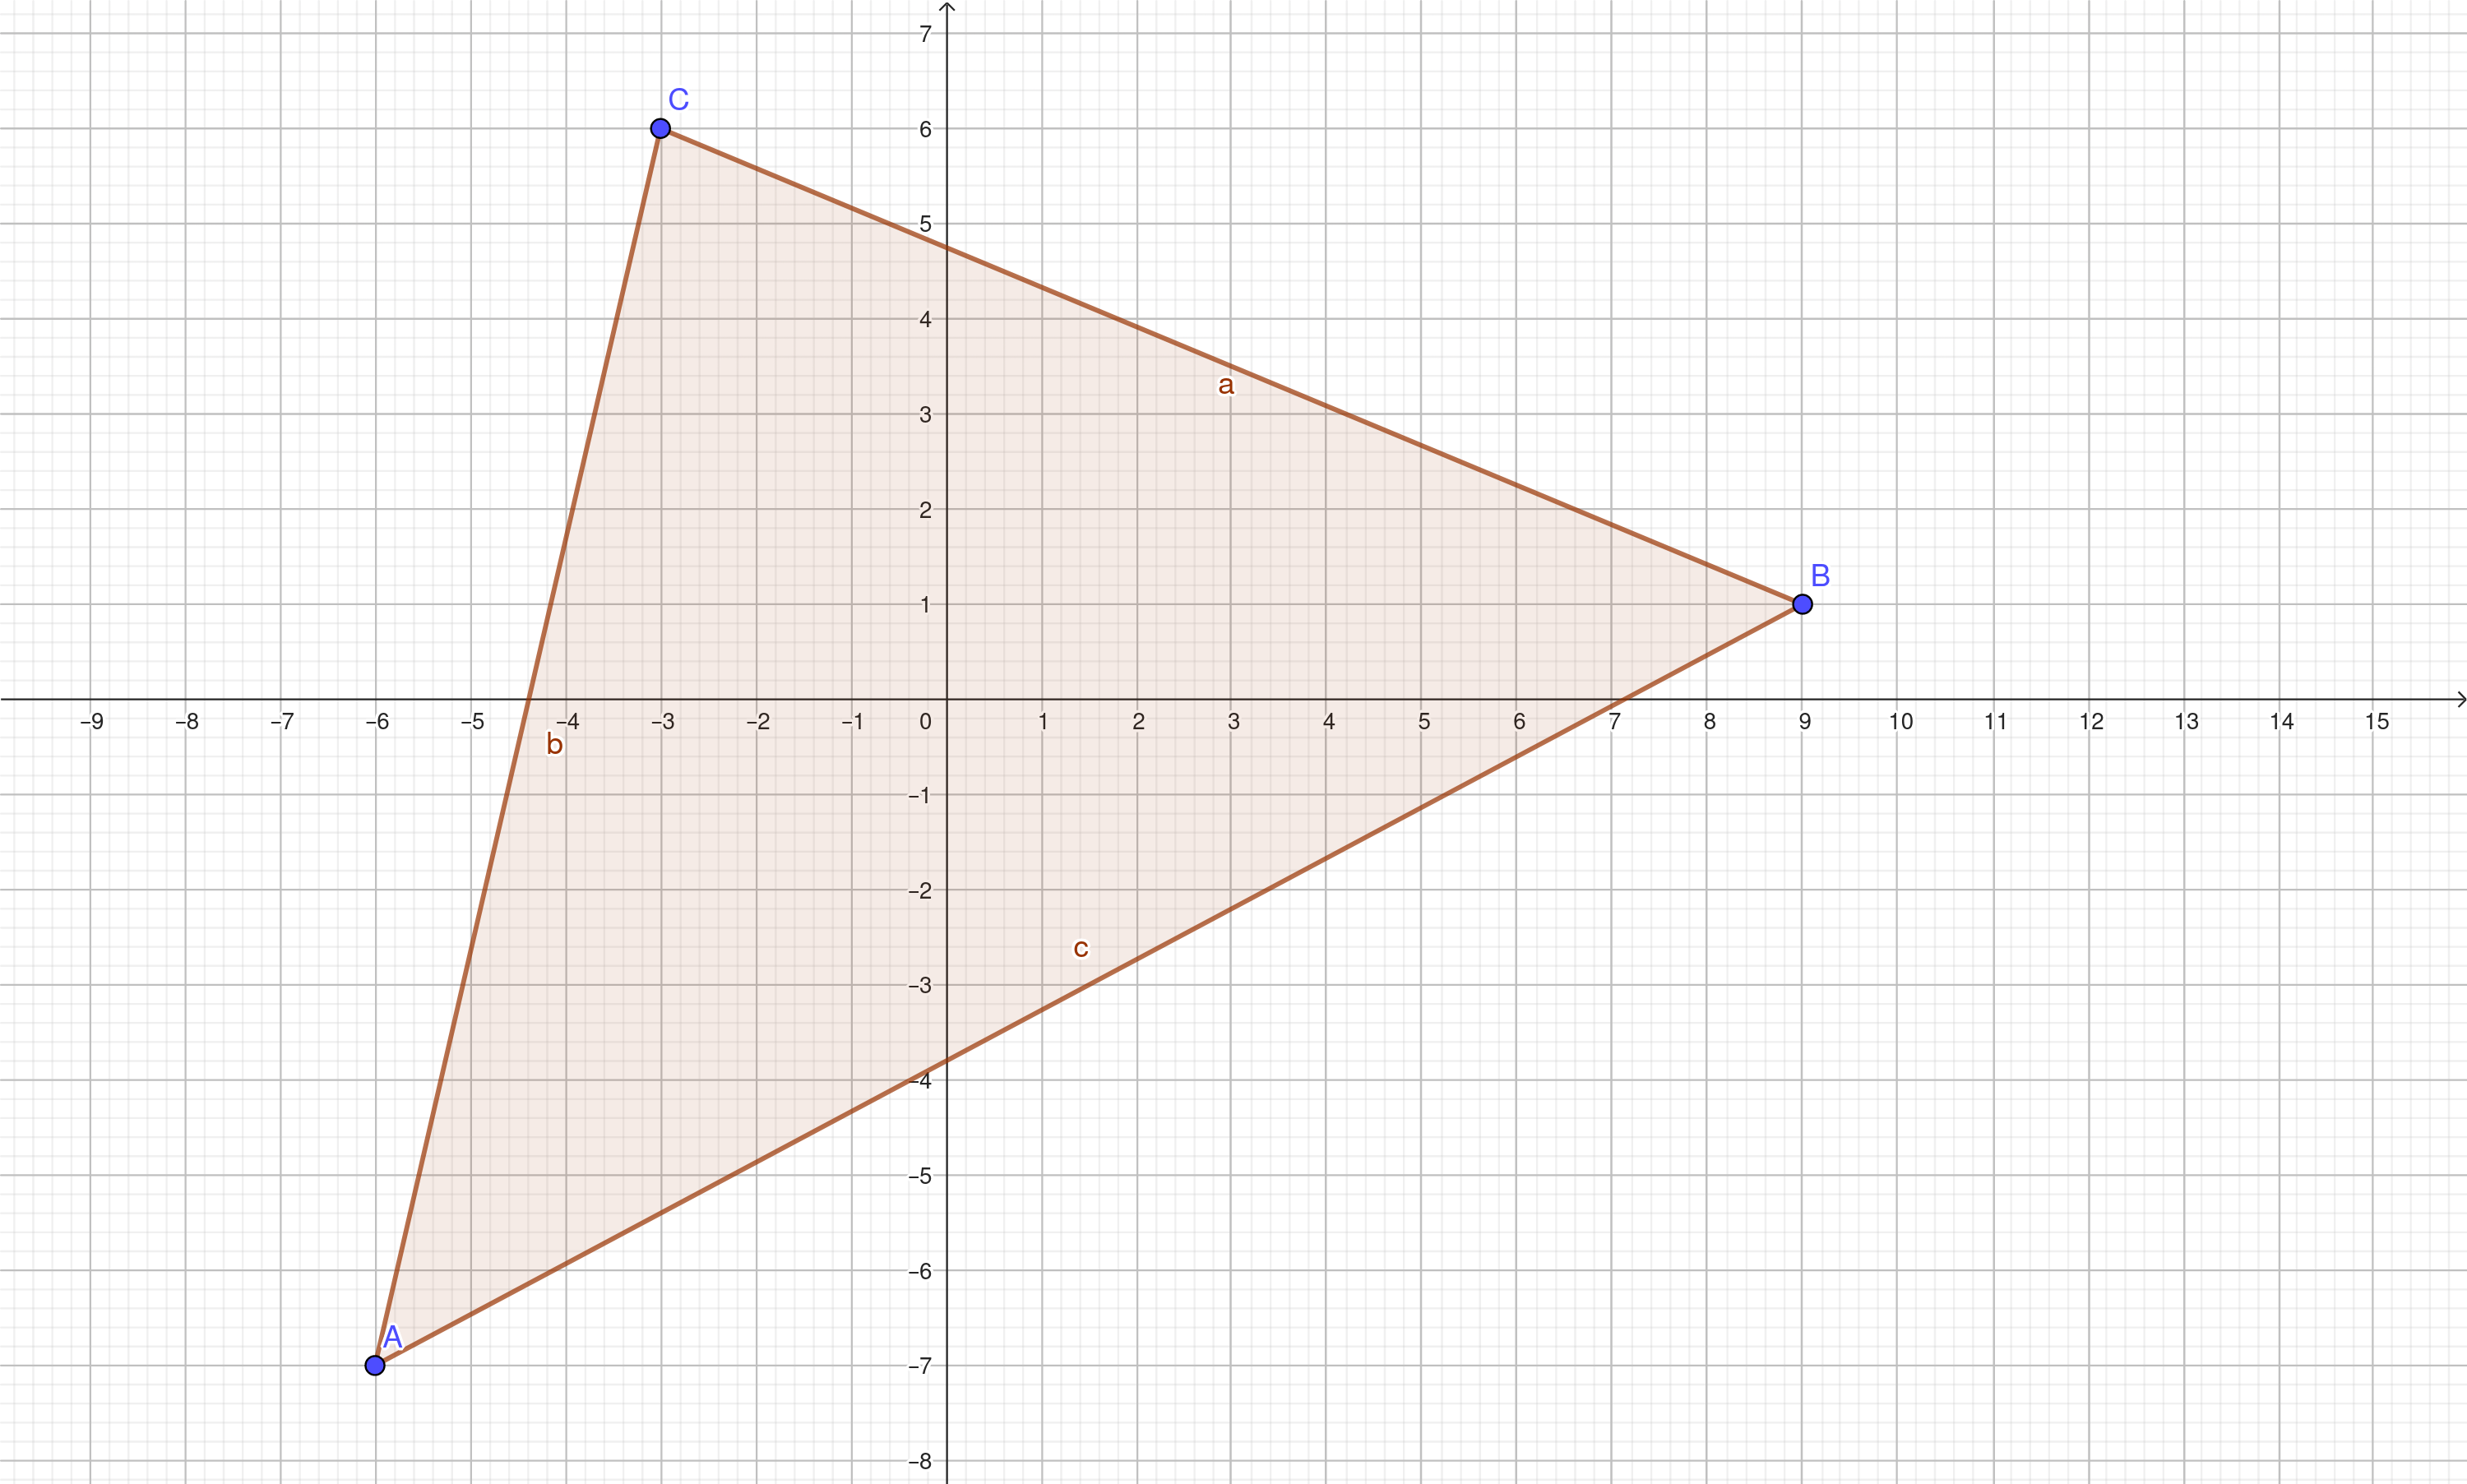
\includegraphics[width=\linewidth]{images/8-29-1.png}

\begin{align}
    \vec{c} &= \vec{AB} \\ 
    &= \AB \\
    c &= |\vec{c}|  \\
    &= 17cm \\[20pt]
    \vec{a} &= \vec{BC} \\
    &= \BC \\
    a &= |\vec{a}| \\
    &= 13cm \\[20pt]
\end{align}

\begin{align}
    \cos({\beta}) &= \frac{\vec{a} \cdot \vec{c}}{|\vec{a}| * |\vec{b}|} \\
    &= \frac{\AB * \BC}{13 * 17}  \\
    &= -\frac{140}{221} \\
    &= \cosval \\[20pt]
    \beta &= \arccos(\cosval) \\
    &\approx \cosang^\circ \\[20pt]
    A &= \frac{a * c * \sin({\beta})}{2} \\
    &= \frac{13 * 17 * \sin({\cosang^\circ})}{2} \\
    &\approx 85.5cm^2
\end{align}

\pagebreak

\paragraph{Answer:}
The obtuse value of $\beta$ ($\cosang^\circ$) was used instead of the acute value of $\beta$ 
($\cosanginv^\circ$). This didn't affect the result because 
$\sin(\beta)$ returns the same value for the obtuse and the acute value of $\beta$


\begin{align}
    \sin(\alpha) &= \sin(180^\circ - \alpha) \\[20pt]
    \sin(\cosang^\circ) &= \sinofang \\
    \sin(\cosanginv^\circ) &= \sinofanginv 
\end{align}
